\newif\ifthesis \thesistrue
\newif\ifpublish \publishfalse

\documentclass[12pt]{article}
\bibliographystyle{apalike}

\usepackage{listings}
\lstset{
  basicstyle=\small\ttfamily,
  frame=lrtb,
}
\lstdefinelanguage{pseudo}{
  keywords={return, if, elif, match, function, for, in, else, and, or, <-, with},
  keywordstyle=\color{blue}\bfseries,
  identifierstyle=\color{black},
  sensitive=false,
  comment=[l]{//},
  morecomment=[s]{/*}{*/},
  commentstyle=\color{purple}\ttfamily,
  stringstyle=\color{red}\ttfamily,
  morestring=[b]"
}
\lstdefinelanguage{Scheme}{
  morekeywords=[1]{define, define-syntax, define-macro, lambda, define-stream, stream-lambda},
  morekeywords=[2]{run, fresh, conde,
    begin, call-with-current-continuation, call/cc,
    call-with-input-file, call-with-output-file, case, cond,
    do, else, for-each, if,
    let*, let, let-syntax, letrec, letrec-syntax,
    let-values, let*-values,
    and, or, not, delay, force,
    quasiquote, quote, unquote, unquote-splicing,
    map, fold, syntax, syntax-rules, eval, environment,  },
  morekeywords=[3]{import, export},
  alsodigit=!\$\%&*+-./:<=>?@^_~,
  sensitive=true,
  morecomment=[l]{;},
  morecomment=[s]{\#|}{|\#},
  morestring=[b]",
  basicstyle=\small\ttfamily,
  keywordstyle=\bf\ttfamily\color[rgb]{0,.3,.7},
  commentstyle=\color[rgb]{0.133,0.545,0.133},
  stringstyle={\color[rgb]{0.75,0.49,0.07}},
  upquote=true,
  breaklines=true,
  breakatwhitespace=true,
  literate=*{`}{{`}}{1}
}
%packages!
\usepackage{comment}
\usepackage{setspace}
\usepackage{datetime}
\usepackage{array}
\usepackage{color}
\definecolor{lightgray}{rgb}{.9,.9,.9}
\definecolor{darkgray}{rgb}{.4,.4,.4}
\definecolor{purple}{rgb}{0.65, 0.12, 0.82}
\usepackage{anyfontsize}
\usepackage{hyperref}
\usepackage{tikz}
\usepackage{graphicx}
\usepackage{titlesec}
\usepackage{geometry}
\usepackage[document]{ragged2e}
\usepackage{parskip}
\usepackage{fancyhdr}
\usepackage{enumitem}
\usepackage{caption}
\DeclareCaptionFormat{myformat}{\footnotesize\selectfont#1#2#3}
\captionsetup{justification=raggedright, singlelinecheck=false, format=myformat}
\usepackage{layout}
\RequirePackage{csquotes}
\RequirePackage{xpatch}
\RequirePackage[
    datamodel=xamkbibdm,
    backend=biber,
    bibstyle=authoryear,
    citestyle=authoryear,
    dashed=false,
    uniquename=init,
    giveninits=true,
    labeldate=long,
    urldate=long,
    dateabbrev=false,
    defernumbers=true,
    maxnames=2,
    maxbibnames=99,
    ]{biblatex}
\setlength\bibitemsep{0.5\baselineskip}
\setlength\bibhang{0pt}

% Biblatex bibliography format modifications
\renewbibmacro{in:}{} % Beware of titles with "In:"
\DeclareNameAlias{sortname}{family-given}
\renewcommand*\finalnamedelim{\addspace\&\addspace}
\DeclareFieldFormat{titlecase}{#1}
\DeclareFieldFormat{editortype}{\mkbibparens{#1}\nopunct}
\xpatchbibmacro{bbx:editor}{\addcomma\space}{\space}{}{}
\DeclareLabeldate{
    \field{date}\field{year}\field{eventdate}\field{origdate}\literal{No date}}
\xpatchbibmacro{date+extrayear}
    {\printtext[parens]}
    {\setunit*{\addperiod\addspace}\printtext}{}{}
\xpatchbibmacro{date+extradate}
    {\printtext[parens]}
    {\setunit*{\addperiod\addspace}\printtext}{}{}
\DeclareFieldFormat{lastmoddate}{Updated #1}
\DeclareFieldFormat{url}{Available at: \url{#1}}
\DeclareFieldFormat{pages}{#1}
\DeclareFieldFormat{urldate}{\mkbibbrackets{Accessed #1}}
\DeclareFieldFormat{title}{#1}
\DeclareFieldFormat[article]{title}{#1}
\xpretobibmacro{url+urldate}{
    \iffieldundef{doctype}%
        {\iffieldundef{url}{}{WWW document. }}
        {\printfield{doctype}\setunit*{\addperiod\addspace}}
    \iffieldundef{lastmodyear}
        {}%
        {\printlastmoddate\setunit*{\addperiod\addspace}}%
}{}{}

\providecommand\phantomsection{}

\addbibresource{uni.bib}

%Setting the font
\renewcommand{\rmdefault}{phv} % Arial
\renewcommand{\sfdefault}{phv} % Arial

%Enter parameters here
\newcommand{\myauthor}{Khoa Vo}
\newcommand{\mytitle}{\ifthesis Functional style within logic programming \else Firewall analysis assistant in miniKanren \fi}
\newcommand{\subtitle}{\ifthesis A miniKanren perspective \else \fi}
\newcommand{\rpas}{\ifthesis Bachelor's thesis \else Report \fi}
\newcommand{\degree}{Degree programme in Information Technology}
\newcommand{\course}{\ifthesis \else Advanced Sever Development Project \fi}

%Line spacing is 1.5
\linespread{1.5}

%Redefining maketitle
\renewcommand{\maketitle}{
\thispagestyle{empty}
\newgeometry{right=2cm, left=2cm, top=4cm, bottom=2cm}

\begin{center}

\fontsize{16}{19} \selectfont \myauthor

\vspace{20pt}

\MakeUppercase{\fontsize{24}{30}\selectfont\mytitle} \\
\fontsize{20}{25}\selectfont\subtitle

\vspace{20pt}

\ifthesis
\fontsize{16}{19} \selectfont {\rpas \\ \degree}
\else
\fontsize{16}{19} \selectfont {\rpas \\ \course}
\fi

\vspace{20pt}

\the\year

%Adding the logo
\vspace{100pt}

\includegraphics{figures/logo.jpg}

\end{center}

%Making the cover background
\tikz[remember picture,overlay] \node[inner sep=0pt] at (current page.center){

\includegraphics[width=\paperwidth,height=\paperheight]{figures/coverbg.png}};
\clearpage
}

%Formatting The sections:
\titleformat{\section}
{\bfseries}
{\thesection}
{.17in}
{\MakeUppercase}

%The subsection:
\titleformat{\subsection}
{\bfseries}
{\thesubsection}
{.17in}
{}

%Formatting the paragraphs
%Put new line between paragraphs
\setlength{\parskip}{\baselineskip}
%No indentation
\setlength{\parindent}{0pt}

%Content of the document
\begin{document}
%The cover page
%First we must clear up the margin
{\maketitle}

%Abstract & Table of content:
\ifthesis\newgeometry{right=2cm, left=2cm, top=2cm, bottom=2cm}
\thispagestyle{empty}

\begin{figure}[t]
    
\includegraphics[height=1.3cm]{figures/logo.jpg}
\end{figure}

\newdateformat{monthyeardate}{%
  \monthname[\THEMONTH] \THEYEAR}
\newcolumntype{A}{>{\singlespacing}m{\linewidth}}

\begin{table}
\begin{tabular} {|l|l|l|l|}
    \hline
    \multicolumn{2}{|l|}{\textbf{Author}} & \textbf{Degree} & \textbf{Time} \\
    \multicolumn{2}{|l|}{} & & \\
    \multicolumn{2}{|l|}{Khoa Vo} & Bachelor or Information Technology & \monthyeardate\today \\
    \hline
    \multicolumn{2}{|l|}{\textbf{Thesis title}} & \textbf{Pages} & \textbf{Appendices} \\
    \multicolumn{2}{|l|}{} & & \\
    \multicolumn{2}{|l|}{Logic Programming in miniKanren} & XX & X \\
    \hline
    \multicolumn{4}{|l|}{\textbf{Commissioned by}} \\
    \multicolumn{4}{|l|}{} \\
    \multicolumn{4}{|l|}{Self initiative} \\
    \hline
    \multicolumn{4}{|l|}{\textbf{Supervisor}} \\
    \multicolumn{4}{|l|}{} \\
    \multicolumn{4}{|l|}{Timo Hynninen} \\
    \hline
    \multicolumn{4}{|l|}{\textbf{Abstract}} \\
    \multicolumn{4}{|A|}{This page is a model for the English thesis abstract. Its length should not exceed one page, and therefore, it may be written with single spacing. The font is Arial, font size 12, and the text typically has 3 to 5 paragraphs, each preceded by an empty line.} \\
    \multicolumn{4}{|A|}{The page begins with identification data in the correct fields, as presented in this template: author’s name, official name of Degree, month and year of approval, supervisors’ names with the official job titles (supervising teacher, the company name or the company’s representative, if the study was commissioned), number of pages from the title page to the end of the list of references / list of figures or tables, and the number of appendices. The first word in the title has capital initial. Otherwise, the title has lower-case initial letters, except for words that are capitalized for grammatical reasons.} \\
    \multicolumn{4}{|A|}{The abstract is a concise, independent account of the thesis content. It has about 200−250 words that summarize the main content. The text introduces the purpose, methods and key results and conclusions. Background information is not included, unless it is especially relevant for fully understanding the text without reading any other parts of the thesis. The text should not refer to any pages of the study, nor figures, tables or equations.} \\
    \multicolumn{4}{|A|}{The abstract is written in past tense, and passive voice (x was studied) and third person (this study examined) should be preferred over personal pronouns (I, we): First, the text introduces the aim of the study (The objective of the thesis was to...). Second, it explains the research method in general terms. (Qualitative methods were used to...). Finally, the text ends with the key results and conclusions (The study showed that...). This part can also discuss whether the thesis succeeded in achieving the goals set.} \\
    \multicolumn{4}{|A|}{The page ends with a field for 3 to 5 keywords accurately describing the thesis content.} \\
    \hline
    \multicolumn{4}{|l|}{\textbf{Keywords}} \\
    \multicolumn{4}{|l|}{} \\
    \multicolumn{4}{|l|}{programming, logic} \\
    \hline
\end{tabular}
\end{table}
\else\fi
\newgeometry{right=2cm, left=2cm, top=2cm, bottom=2cm}
\thispagestyle{empty}
{\tableofcontents}

\newpage

%Body layout
\newgeometry{right=2cm, left=4.3cm, top=2.25cm, bottom=1.25cm}
\pagestyle{fancy}
\fancyhf{}
\renewcommand{\headrulewidth}{0pt}
\fancyhead[C]{\thepage}

%The below line was marked with "b"
%===========================================================================================================
%CONTENT GOES HERE!
\lstset{language=Scheme, showstringspaces=false,  breaklines=true}

\ifpublish
    \section{Introduction}

To begin, let us take a look at a particular logic puzzle:

{\small\textit{"On a certain fictional island there are only two types of inhabitants: the knights always tell the truth, and the knaves who always tell lies. One day, a logician pays a visit to a small family of three on the island. While the four are having dinner, the logician asks whether the dad is a knight or a knave. The dad says "Ask my son and he will tell you the truth". The son then says "We are all of the same type". Finally, the mom says "You have to excuse us, one of them cannot tell the truth". Can you tell which family members are knight, and which are knaves?"}}

If the dad is telling the truth, then the son's statement is true and so the entire family are knights. However, that must mean the mom is also telling the truth, and they cannot all be knights (a contradiction). Therefore, the dad must be lying, and so is the son. Following from the son's lie it must be the case that the family has both types of people. Since two family members are already determined to be knaves, the mom must be a knight.

What if we start first from the mom? Suppose she is telling lies, then both the son and dad are telling the truth. However, the son's statement must be wrong since the family is mixed (a contradiction). Therefore, the mom must be telling the truth, and either the dad or the son is lying (or both). If the son is telling the truth, then it immediately follows he is lying, since according to him the dad must be telling the truth and the mom's statement now cannot be true. Therefore, the son is lying and so is the dad for referring to him. This conclusion is consistent with the first approach.

This type of logic puzzle was popularized by (\cite{knight}). In the solving of the puzzle, we can see a relatively simple mechanism in action. First, determine one possible value of an unknown variable (if there is none left, abandon the branch). Second, check if the state is logically consistent; if yes, loop back to the first step; if no, undo the choice made in the first step, choose something else, and carry on with the algorithm. The process terminates either when there is no longer any choice to be made, in which case we can output the answer, or when we have exhausted all possibilities and no choice can lead to a consistent state.

Every time a person wants to roll out a program to solve a puzzle of similar kinds, they need to not only specify the problem, but also write the backtracking algorithm as well. After a while, one would wish that the second part of the task -- having little to do with the problem -- should be standardized (and optimized) by some sort of framework, so that only the problem needs to be defined. \textbf{Logic programming} promises to make this job easier for those people (and hopefully for everyone else as well). Using a language of this kind, the programmer only needs to declare rules, and the computer will give them back all states consistent within those rules. One such language which will be discussed in this text is \textbf{miniKanren}.

miniKanren is neither the only or the first logic programming language. The idea dates back to 1972, when Prolog was first invented by Alain Colmerauer and Phillipe Roussel. The name Prolog was an abbreviation for \textbf{pro}grammation en \textbf{log}ique. Despite the name, Prolog users generally do not shy away from its extra-logical features. These features on one hand can enhance greatly performance, but they can also make programs less declarative, incomplete and even unsound. (\cite{early-prolog})

Prolog was once considered the future of computing, at least in Europe and especially in Japan. In the 1970's, the Japanese International Trade and Industry (MITI) wanted to take over the computer industry with a new Fifth Generation Computing System Project (named ICOT). The project failed, however, because the language was not fast enough to compete with other mainstream object-oriented languages like Java and C\#. Carl Hewitt summed it up nicely with: "\textit{Computation is not subsumed by deduction.}" (\cite{logic-fail})

In this paper we do not talk about performance, but instead focus on the logic. Relational programming is a discipline of logic programming whereby extra-logical features that provide unsound behavior are not used. This guarantees that all answers are returned even when non of the arguments are grounded. The design philosophy of miniKanren puts great emphasis on this discipline\footnote{"Kanren" is literally Japanese for "relation".}. (\cite{byrdphd})

miniKanren does not have its own interpreter, but is embedded in a larger programming language. One such language -- which we will use in this paper -- is Scheme. Scheme is our implementation of choice for three reasons. The first reason is that it is the canonical version mentioned in almost every academic paper written on the language. The second reason is that Scheme's macro makes the syntax less clunky and more natural to read and write. Last but not least, Scheme is an extremely elegant language with minimal syntax (some would even say no syntax), hence it is trivial to briefly specify a small portion of the language to be used in this text.

The layout of this paper is as follow: Section ... will specify a subset of Scheme. Section ... discusses miniKanren. Finally, a firewall design assistant -- one of the main real-world application in this paper -- is given in section ....
    \section{PRELIMINARIES}
\label{prelim}
This section gives a brief overview to miniKanren.
A complete introduction to the language is presented in \textcite{reasoned}.
\textcite{byrdphd} gives an excellent dissertation on the implementation details, but for readers who are either interested in a more fundamental treatment of logic programming, or just find Scheme macros difficult to comprehend, the implementation in \textcite{micro} is perhaps more suitable. Alas, this thesis assume familiarity with Scheme, to which the introduction can be found in \textcite{sicp} and \textcite{tspl4}.

\subsection{Basic concepts of miniKanren}
As mentioned earlier miniKanren is not a standalone programming language but an embedded structure inside a language (in our case, Scheme). Language components from the low-level perspective include the following:
\begin{itemize}
\item \textbf{Logic variables}: It is important to distinguish these from naming variables. Unbound naming variables always mean that an error has occurred. In contrast, unbound logic variables are perfectly valid objects. From here on, variable means logic variable unless stated otherwise.
\item \textbf{Streams}: Streams are simply lazy lists that will yield values only when we ask for them (\cite{sicp}). This laziness can be used to represent an infinite number of answers with finite computational resources.
\item \textbf{States} (also \textbf{packages}): State is the most important object in miniKanren. A state is what keeps track of all logical assertions made by the program.
\item \textbf{Goal}: A goal is a function mapping a state to a stream of states. Goals should only be created by \textbf{goal constructors}, as will be discussed below.
\item \textbf{Relation}: Relations are simply Scheme functions that return goals.
\item \textbf{Program}: Every miniKanren program consists of a goal wrapped inside of the \code{run} form which, with the help of zero or more relation definitions, outputs a list of answers, which can be thought of as normalized and pretty-printed states.
\end{itemize}

We can also analyze the language from a high-level point of view in terms of its primitives, its means of combination, and its means of abstraction (\cite[359]{sicp}). miniKanren's primitives are \textbf{logical constraints} and a special form to create and bind new logic variables. Its two means of combination are conjunction and disjunction. Its only means of abstraction is relation.

\code{run} is the interface converting goals to programs which produce answers. To do this, \code{run} catches the stream of states produced by the goal and turns it into a list of specified length. In the process, it also converts these states into a more readable format -- a process called \textbf{reification} -- which also highlights the values of \textbf{query variables}. This thesis will not describe precisely what the format produced by reification is, but it can be intuitively grasped when more examples are introduced. Meanwhile, readers need only know that \code{run} has the following syntax:
\begin{lstlisting}
(run <answer-count> (<query-var-1> <query-var-2> ...) <goal>)
\end{lstlisting}

Additionally, users can use the following form to get back all answers regardless of how many there are:
\begin{lstlisting}
(run* (<query-var-1> <query-var-2> ...) <goal>)
\end{lstlisting}

\subsection{Core primitives: equality and fresh variable creation}
The most important goal constructor (primitive constraint) is \code{==}.
Simply put, \code{==} unifies (declares equality of) two terms. More precisely, \code{==} receives a state and returns a stream. This stream can either contain one state where the two terms become their most general unifier, or be empty when they cannot be unified.

Actually, \code{==} is the only constraint in the what is called the "core" of miniKanren. Even with only this constraint, the language is already Turing-complete. However, none but the simplest programs can be written conveniently using \code{==}.

The examples below introduce some uses of \code{==}.
\begin{lstlisting}
(run* (q)
  (== 'x 'x))
\end{lstlisting}
$\Rightarrow$ \code{(_.0)}

\begin{lstlisting}
(run* (q)
  (== '(x y) '(x y)))
\end{lstlisting}
$\Rightarrow$ \code{(_.0)}

\begin{lstlisting}
(run* (q)
  (== 'x 'y))
\end{lstlisting}
$\Rightarrow$ \code{()}

In the first and second examples, the two arguments to \code{==} are already equal. Hence the program returns one successful answer. In the third example, the two terms \code{x} and \code{y} can never be unified and the program returns the empty list indicating that there is no possible answer. In these cases, \code{==} is only used to compare terms. \code{==} becomes a lot more interesting when variables are involved.

To make logic variables, we must use the goal constructor (fresh variable creator) \code{fresh}. \code{fresh} is perhaps the most complex goal constructor in miniKanren, partly because it is also a special syntactic form. Operationally, \code{fresh} creates one or more fresh logic variables. Syntactically, \code{fresh} also bind these newly created variables to identifiers within its body.

Let us take a look at some examples involving \code{fresh}:

\begin{lstlisting}
(run* (q)
  (fresh (v)
    (== v 'x)
    (== q v)))
\end{lstlisting}
$\Rightarrow$ \code{(x)}

\begin{lstlisting}
(run* (q)
  (fresh (v u)
    (== v 'x)
    (== u v)
    (== q u)))
\end{lstlisting}
$\Rightarrow$ \code{(x)}

The first program introduces a new logic variable \code{v} which is then unified with both the symbol \code{x} and the query variable \code{q} (the order does not matter). The only answer returned is the value of \code{q}, which is the symbol \code{x}. In the second program, two variables are introduced. Since \code{u} is unified with \code{v} and the rest of the program is the same, the answer is also the same.

Unlike Prolog, we cannot refer to a logic variable not introduced by, or not in the body of \code{fresh}. For example, the call below fails.
\begin{lstlisting}
(run* (q)
  (fresh (v)
    (== q v)  ; Perfectly fine
    (== q u)  ; Error: variable u is unbound
  )
  (== q v)  ; Error: variable v is unbound
)
\end{lstlisting}
The term "variable" in the error messages refers to naming variables, not logic variables. Technically speaking, logic variables need not even have names. When talking about "the variable \code{v}", we actually mean "the logic variable bound to the naming variable \code{v}". The last example below showcases lexical scope created by \code{fresh}.
\begin{lstlisting}
(run* (q)
  (fresh (v)
    (== v 'x)
    (== q v)  ; v bound to the symbol x
    (fresh (v)
      (== v 'y)
      (== q v)  ; v bound to the symbol y
      )))
\end{lstlisting}
$\Rightarrow$ \code{()}

This call fails because \code{q} was unified to two logic variables having two different values. They are just happen to be bound to the same naming variable \code{v}. The first \code{v} is introduced by the outer \code{fresh}, the second \code{v} is introduced by the inner \code{fresh} and \textbf{shadows} the outer \code{v}. Although shadowing seems to be a confusing thing in this example, it becomes useful especially when writing larger programs.

For our purpose, it is important to demystify the answer format returned by miniKanren (more precisely, by \code{run}). First, unknown variables declared to be the same (e.g. by \code{==}) always have the same index, for instance:
\begin{lstlisting}
(run* (p q r) (== p q))
\end{lstlisting}
$\Rightarrow$ \code{((_.0 _.0 _.1))}

Second, if a variable is tied to a value, the value will be used instead of the form \code{_.n}. Furthermore, if a variable is sure to be a pair, that fact is also made known in the answer, as the following example shows:
\begin{lstlisting}
(run* (q) (fresh (x y) (== `(,x ,y) q)))
\end{lstlisting}
$\Rightarrow$ \code{((_.0 _.1))}

A simple principle to keep in mind is that \textit{information must be preserved during reification}. The only lost information, however, is the names of logic variables. The reason for that is due to the name conflict phenomenon mentioned earlier; that is, if we were to simply represent unknown variables by their names, there would be no way of telling whether two variables were really declared to have the same value or they just happen to bear the same name. As we shall see later, staticKanren uses a simple technique to recover names of unbound variables using birthdate tags.

\subsection{Goal combinators: disjunction and conjunction}
Next, we take a look at the goal constructor (goal disjunction combinator) \code{conde}.
If one needs to point out exactly one thing that makes logic programming seem magical, disjunction would be a good answer. Every example above returns either zero or one answer. With \code{conde}, we can start returning two or more answers. The \code{conde} form consists of a number of \textbf{clauses}, each containing a number of goals, for example:

\begin{lstlisting}
(run* (q)
  (conde
    [(== 'x q)]
    [(== 'y q)]))
\end{lstlisting}
$\Rightarrow$ \code{((x y))}

As promised, this program actually returns two answers. We can view \code{conde} as creating two "parallel universes" where \code{q} is unified with \code{x} in the first and \code{y} in the second.

The final goal constructor (goal conjunction combinator) of core miniKanren does not actually exist. However, we have already encountered conjunction multiple times in the previous examples. Intuitively, conjunction is implicit whenever two or more goals are written in series in the bodies of \code{run}, \code{fresh} or \code{conde} clauses. Each of the examples below returns \code{()} due to value conflict.
\begin{lstlisting}
(run* (q)
  (conde
    [(== 'x q) (== 'y q)]))
\end{lstlisting}

\begin{lstlisting}
(run* (q)
  (== 'x q)
  (== 'y q))
\end{lstlisting}

\begin{lstlisting}
(run* (q)
  (fresh ()
    (== 'x q)
    (== 'y q)))
\end{lstlisting}

\subsection{Disequality}
The introduction of miniKanren's core should be complete with \code{==}, \code{fresh}, \code{conde} and conjunction. However, we will also take a look at the most important extra constraint \code{=/=}. As the name suggest, \code{=/=} declares \textbf{disequality} of two miniKanren terms. A small example is given below:
\begin{lstlisting}
(run* (q) (=/= 5 q))
\end{lstlisting}
$\Rightarrow$ \code{((_.0 (=/= ((_.0 5)))))}

The program above returns one answer, stating that while \code{q} is unknown, it must not be made equivalent to \code{5}. If that happens to be the case, the program fails, as shown in the following case:
\begin{lstlisting}
(run* (q) (=/= 5 q) (== q 5))
\end{lstlisting}
$\Rightarrow$ \code{()}

To better understand answers containing disequalities, a more complex example is needed, such as the following:
\begin{lstlisting}
(run* (q p r) (=/= `(,q ,p) `(1 2)) (=/= p r))
\end{lstlisting}
$\Rightarrow$
\code{(((_.0 _.1 _.2) (=/= ((_.0 1) (_.1 2)) ((_.1 _.2)))))}

The above answer shows see that each disequality constraint store, as presented in the answers, is a list of mini anti-substitution lists. Each anti-substitution list, in turn, contains disassociations of the form \code{(x v)} where \code{x} must be a variable. Failure happens when all disassociated terms in one anti-substitution list are equal. In plain English, the answer above says that \code{p} is different from \code{r} and that either \code{q} must be different from \code{1} or \code{p} must be different from \code{2}, which is exactly what we declared in the program.
    \ifthesis \section{Relational conditionals with pseudo-functions}\label{reif}
\subsection{The problem with conde}
Suppose we need to write a relation called \code{lookupo} to retrieve a variable's value in an environment. The task at first is just a straightforward transformation from the Scheme function \code{lookup}.
\begin{lstlisting}
(define lookup
  (lambda (x env)
    (let ([a (car env)])
      (cond
       [(eq? x (lhs a)) (rhs a)]
       [else (lookup x (cdr env))]))))

(define lookupo
  (lambda (x env t)
    (fresh (y b rest)
      (== `((,y ,b) . ,rest) env)
      (conde
       [(== y x) (== b t)]
       [(=/= y x) (lookupo x rest t)]))))
\end{lstlisting}

Later on we might need to actually handle the case where the variable is unbound instead of raising an error or fail. We update both definitions:
\begin{lstlisting}
(define lookup
  (lambda (x env)
    (cond
     [(null? env) #f]
     [else
      (let ([a (car env)])
        (cond
         [(eq? x (lhs a)) a]
         [else (lookup x (cdr env))]))])))

(define lookupo
  (lambda (x env t bound?)
    (conde
     [(== '() env) (== #f bound?)]
     [(fresh (y b rest)
        (== `((,y ,b) . ,rest) env)
        (conde
         [(== y x) (== #t bound?) (== b t)]
         [(=/= y x) (lookupo x rest t bound?)]))])))
\end{lstlisting}

So far so good: \code{lookup} only needs to add an input indicating whether the variable is bound; meanwhile for \code{lookup} we have to devise a special signal, namely \code{#f}, for the unbound case\footnote{There is technically a way to return multiple values in Scheme, but doing so would be lengthy and unconventional.}. However, a problem arises when we actually use the output signal:
\begin{lstlisting}
(define case1
  (lambda (x env)
    (cond
     [(lookup x env) => rhs]
     [else #f])))

(define case1o
  (lambda (x env out)
    (conde
     [(lookupo x env out #t)]
     [(lookupo x env 'unbound #f) (== #f out)])))
\end{lstlisting}

Why can we not use \code{else} in the second clause? The reason is that despite the similarity in appearance, \code{conde} does not process its clauses from top to bottom like \code{cond} does, so there can be no default case. As a result, programmers must always be prepared to append extra denials in lower \code{conde} clauses. This issue gets serious when the control flow is more complex:

\begin{lstlisting}
(define case2
  (lambda (x y env)
    (cond
     [(lookup x env) => rhs]
     [(lookup y env) => rhs]
     [else #f])))

(define case2o
  (lambda (x y env out)
    (conde
     [(lookupo x env out #t)]
     [(lookupo x env '? #f) (lookupo y env out #t)]
     [(lookupo x env '? #f) (lookupo y env '? #f)
      (== #f out)])))
\end{lstlisting}

The example above is still generous, as it is usual for relations to include four or more \code{conde} clauses. The number of extra denials exhibits quadratic growth, introducing opportunities for errors without any significant contribution to the meaning of the program. Fortunately, there is a simple way to deal with them using a technique inspired by \textcite{reif}. This solution relies on \textbf{pseudo-functions}.

\subsection{Pseudo-function and condo}
Pseudo-functions receive their results as arguments instead of returning them. To make sense of this concept, observe the following transformation (the "t" at the end denotes pseudo-functions, simply because it is too late to change):
\begin{lstlisting}
;; From function
(define bar (lambda (in) 'v))
;; To relation
(define baro (lambda (in out) (== out 'v)))
;; To pseudo-function...
(define bart (lambda (in) (lambda (out) (baro in out))))
;; ...which is equivalent to
(define bart (lambda (in) (lambda (out) (== out 'v))))
\end{lstlisting}

From a low-level point of view, a pseudo-function is a function which takes a single argument and return a goal. It can be seen that the act of returning values in functional programming is analogous to the act of unification in logic/relational programming. Moreover, a relation can be made to return whichever of its formal parameters, depending on the circumstances:
\begin{lstlisting}
;; From relation
(define conso (lambda (a d ls) (== `(,a . ,d) ls)))
;; To pseudo-function 1
(define cart (lambda (ls) (lambda (a) (fresh (d) (conso a d ls)))))
;; To pseudo-function 2
(define cdrt (lambda (ls) (lambda (d) (fresh (a) (conso a d ls)))))
;; To pseudo-function 3
(define const (lambda (a d) (lambda (ls) (conso a d ls))))
\end{lstlisting}
I have never encountered a situation where this is actually useful, since there is generally only one parameters deemed as the "output". It is worth noting that even though pseudo-functions act like pure functions, they can affect more than just the output. For instance, the goal \code{((cart x) a)} will always instantiate \code{x} to a pair if it is currently unknown.

Going back to the problem of conditionals, we first define two trivial pseudo-functions \code{truet} and \code{falset}, "returning" \code{#t} and \code{#f} respectively.

\begin{lstlisting}
(define truet (lambda () (lambda (?) (== #t ?))))
(define falset (lambda () (lambda (?) (== #f ?))))
\end{lstlisting}

Next, we define a single "primitive" pseudo-function similar to Scheme's \code{eq?}\footnote{Depending on the implementation, more primitive pseudo-functions may be defined using additional primitive constraints.}. This function relies on both \code{==} and \code{=/=} to correctly express two branches of the output.
\begin{lstlisting}
(define ==t
  (lambda (x y)
    (lambda (?)
      (conde
       [(== #t ?) (== x y)]
       [(== #f ?) (=/= x y)]))))
\end{lstlisting}

Next, we provide ways of creating more complex pseudo-functions from simpler ones, starting with \code{negt} (negation):
\begin{lstlisting}
(define negt
  (lambda (g)
    (lambda (?)
      (conde
       [(== #t ?) (g #f)]
       [(== #f ?) (g #t)]))))
\end{lstlisting}

From this, \code{=/=t} can be trivially derived:
\begin{lstlisting}
(define =/=t
  (lambda (x y) (negt (==t x y))))
\end{lstlisting}

Similarly, \code{conjt} (conjunction) and \code{disjt} (disjunction) are defined using macro:
\begin{lstlisting}
(define-syntax conjt
  (syntax-rules ()
    [(_) (truet)]
    [(_ g) g]
    [(_ g1 g2 gs ...)
     (lambda (?)
       (conde
        [(g1 #t) ((conjt g2 gs ...) ?)]
        [(== #f ?) (g1 #f)]))]))

(define-syntax disjt
  (syntax-rules ()
    [(_) (falset)]
    [(_ g) g]
    [(_ g1 g2 gs ...)
     (lambda (?)
       (conde
        [(== #t ?) (g1 #t)]
        [(g1 #f)  ((disjt g2 gs ...) ?)]))]))
\end{lstlisting}

This next example demonstrates conjunction:
\begin{lstlisting}
(run* (t x y z)
   ((conjt (==t x y)
           (==t y z))
    t))
\end{lstlisting}
$\Rightarrow$
\begin{lstlisting}
(((#f _.0 _.1 _.2) (=/= ((_.0 _.1))))
 (#t _.0 _.0 _.0)
 ((#f _.0 _.0 _.1) (=/= ((_.0 _.1)))))
\end{lstlisting}

Similarly, this example demonstrates disjunction:
\begin{lstlisting}
(run* (t x y z)
   ((disjt (==t x y)
           (==t y z))
    t))
\end{lstlisting}
$\Rightarrow$
\begin{lstlisting}
((#t _.0 _.0 _.1)
 ((#t _.0 _.1 _.1) (=/= ((_.0 _.1))))
 ((#f _.0 _.1 _.2) (=/= ((_.0 _.1)) ((_.1 _.2)))))
\end{lstlisting}

Finally, we can define the goal constructor \code{condo} -- the closest relational counterpart of \code{cond}. Keep in mind that \code{succeed} stands for the "do nothing" goal and \code{fail} stands for the "always fail" goal.
\begin{lstlisting}
(define-syntax condo
  (syntax-rules (else)
    [(_ [else]) succeed]
    [(_ [else g]) g]
    [(_ [else g1 g2 g* ...])
     (fresh () g1 g2 g* ...)]
    [(_ [test g* ...] c* ...)
     (conde
      [(test #t) g* ...]
      [(test #f) (condo c* ...)])]
    [(_) fail]))
\end{lstlisting}
\code{condo} is an interesting combinator because it uses two types of objects, pseudo-functions in the test positions and normal miniKanren goals in the bodies of each clause. The \code{else} keyword can be used to signify the default case; although it can be omitted, in which case the program fails when no clause matches. The example below demonstrates the use of \code{condo}:
\begin{lstlisting}
(run* (x y z)
  (condo
   [(==t x y) succeed]
   [(==t y z) succeed]
   [else (== x z)]))
\end{lstlisting}
$\Rightarrow$
\begin{lstlisting}
((_.0 _.0 _.1)
 ((_.0 _.1 _.1) (=/= ((_.0 _.1))))
 ((_.0 _.1 _.0) (=/= ((_.0 _.1)))))
\end{lstlisting}

We are now able to replace \code{lookupo} with the pseudo-function \code{lookupt}.
\begin{lstlisting}
(define lookupt
  (lambda (x env t)
    (lambda (bound?)
      (conde
       [(== '() env)
        (== #f bound?) (== t 'unbound)]
       [(fresh (y b rest)
          (== `((,y ,b) . ,rest) env)
          (condo
           [(==t y x) (== #t bound?) (== b t)]
           [else
            ((lookupt x rest t) bound?)]))]))))
\end{lstlisting}
Now the comparison between \code{case2} and \code{case2o} does not look so bad anymore.
\begin{lstlisting}
(define case2
  (lambda (x y env)
    (cond
     [(lookup x env) => rhs]
     [(lookup y env) => rhs]
     [else #f])))

(define case2o
  (lambda (x y env)
    (lambda (out)
      (condo
       [(lookupt x env out) succeed]
       [(lookupt y env out) succeed]
       [else (== #f out)]))))
\end{lstlisting}

Some readers may already be convinced to convert all of their relations to pseudo-functions. However, there are still some issues to address. Although hiding the control flow is great for readability, the downside is that there is no simple way to see what is done behind the layer of abstraction. As a result, it becomes easier to accidentally change the behavior of programs. Take for example this goal using \code{condo}:
\begin{lstlisting}
(fresh (x y)
  (condo
   [(==t 'a x) (== 'A y)]
   [(==t 'b x) (== 'B y)]
   [(==t 'c x) (== 'C y)]))
\end{lstlisting}
It is not clear that there is an issue with this code, because it looks so much like normal Scheme. The issue only shows itself when we expand the \code{condo}:
\begin{lstlisting}
(fresh (x y)
  (conde
   [(== 'a x) (== 'A y)]
   [(=/= 'a x) (== 'b x) (== 'B y)]
   [(=/= 'a x) (=/= 'b x) (== 'c x) (== 'C y)]))
\end{lstlisting}
Clearly, the additional denials in these \code{conde} clause are redundant since they are already mutually exclusive. Moreover, switching from \code{conde} to \code{condo} always means changing the way miniKanren's search work.

Reality has shown that serious miniKanren users who are conscious about their programs' behavior cannot afford \code{condo}, so we are once again stuck with lengthy, buggy \code{conde} clauses whose meaning cannot not be easily grasped. The next section addresses this issue by offering a way to verify the correctness of existing programs with \textbf{staticKanren}. \section{staticKanren}\label{static}
This section introduces staticKanren, a language designed to analyze miniKanren programs. We first step through a few simple examples in section \ref{static_intro} to develop intuition for the detailed implementation in section \ref{static_imp}. Section \ref{S} and \ref{au} demonstrate some applications of the language.

\subsection{Introductory examples}\label{static_intro}
On the surface, staticKanren was designed to look as close to miniKanren as possible; however there are still some fundamental differences. Unlike miniKanren, staticKanren cannot deal with infinite answer streams. In fact, staticKanren programs can only return all answers using \code{run*} as there is no point withholding computed answers. As a result, we cannot write non-trivial recursive relations in staticKanren as-is. Looking on the bright side, this gives the language a simpler implementation.

staticKanren offers only three primitives constraints: equality, disequality and \textbf{lazy} constraint. The first two retain their syntax and semantics from miniKanren, whereas the third is a new addition to emulate recursive relations. There is no reason not to include more primitive constraints, the more knowledge staticKanren has, the better answers it can return. However, adding other constraints would be a distraction from our goal. Therefore, only disequality is implemented because it plays such an important role in relational programs.

In staticKanren, answers are also interpreted as programs. For that reason, the language must treat variable names more seriously. For example (in this section, $\Rightarrow$ means "evaluating under staticKanren"):


\begin{lstlisting}
(run* (q p) (== q 4))
\end{lstlisting}
$\Rightarrow$ \code{(((4 #(p 0)) () ()))}

If the program above were run under miniKanren instead, the answer would have been \code{((4 _.0))}. The variable \code{p} remains unknown in the answer, so it gets to keep its name (let us ignore the zero on the right for now). Besides the query variables, staticKanren always returns two additional constraint stores, one for disequalities and one for fake constraints. Hence, every answer has the same shape of a three-element list.  The next example demonstrates how the language deals with name shadowing:

\begin{lstlisting}
(run* (q a) (fresh (a d) (== q `(,a . ,d))))
\end{lstlisting}
$\Rightarrow$ \code{((((#(a 1) . #(d 1)) #(a 0)) () ()))}

The same program under miniKanren would return \code{(((_.0 . _.1) _.2))} instead. There are two variables having the same name \code{a}. staticKanren can still distinguish these two variables by their \textbf{birthdate} (the number shown on the right). Meanwhile, miniKanren sidesteps this problem completely by introducing a new name for every unbound variables used in the answer. It is perhaps a subjective matter to debate which representation is better, but there is one at least one theoretical problem avoided by the new approach\footnote{This example was even mentioned in one of the online miniKanren's Uncourse Hangouts organized by William Byrd.}:

\begin{lstlisting}
(run* (q p) (== q '_.0))
\end{lstlisting}
$\Rightarrow$ \code{(((_.0 #(p 0)) () ()))}

The same program under miniKanren would return \code{((_.0 _.0))}!. And because two Scheme symbols are the same iff they look the same, there is no way to distinguish \code{p} and \code{q} in that case, even from the computer's perspective. The last example demonstrates fake constraints. It is a silly program to stress that these fake constraints have no actual meaning, as the \code{fake} form does no more than evaluating its body and add the resulting expression to the fake constraint store.
\begin{lstlisting}
(run* (q p r) (fake `(mother ,q ,p)) (fake `(father ,p ,r))))
\end{lstlisting}

$\Rightarrow$
\begin{lstlisting}
(((#(q 0) #(p 0) #(r 0))
 ()
 ((father #(p 0) #(r 0)) (mother #(q 0) #(p 0)))))}
\end{lstlisting}



\subsection{Implementation}\label{static_imp}
This section presents an R6RS compliant implementation of staticKanren. We will highlight only those parts that demonstrates fundamental differences from the standard miniKanren implementation describe by \textcite{byrdphd}\footnote{However, this does not mean that merely overriding the definitions of miniKanren by the ones in this paper would give a working staticKanren since there are many other small technical differences.}. The full implementation can be found at \url{https://github.com/lackhoa/staticKanren}.

The following functions construct and dispatch variables. Variables are vectors of two elements: its name (a symbol) and its birthdate (a number). Additionally, we would like to create a total order on the set of variables. A variable is prioritized over another if its birthdate is less (i.e. it was introduced sooner), or if it has the same birthdate and a lexicographically lesser name. We call prioritized variables \textbf{seniors} and less prioritized ones \textbf{juniors}.
\begin{lstlisting}
(;; name is a symbol, bd is a number
 define var (lambda (name bd) (vector name bd)))
(define var->name (lambda (var) (vector-ref var 0)))
(define var->bd (lambda (var) (vector-ref var 1)))
(define var? vector?)
(define var<?
  ;; v1 is prioritized over v2
  (lambda (v1 v2)
    (let ([n1 (symbol->string (var->name v1))] [bd1 (var->bd v1)]
          [n2 (symbol->string (var->name v2))] [bd2 (var->bd v2)])
      (or (< bd1 bd2)
          (and (= bd1 bd2) (string<? n1 n2))))))
\end{lstlisting}

Next we have definitions about constraints. Many of the functions could easily be defined automatically using record, but we use list to retain conceptual simplicity and flexibility. A constraint is a 4-tuple consisting of a substitution \code{S}, a date counter \code{C}, a disequality store \code{D} and a fake constraint store \code{F}. The counter starts from 0 and only goes upwards. Additionally, \code{letg@} is a special form to dispatch on states.
\begin{lstlisting}
(define all-constraints '(S C D F))
(define init-S '())
(define init-C 0)
(define init-D '())
(define init-F '())
(define make-c (lambda (S C D F) (list S C D F)))
(define init-c (make-c init-S init-C init-D init-F))
(define c->
  (lambda (c store)
    (rhs (assq store (map list all-constraints c)))))
(define update-S (lambda (c S) (letg@ (c : C D F) (make-c S C D F))))
(define update-C (lambda (c C) (letg@ (c : S D F) (make-c S C D F))))
(define update-D (lambda (c D) (letg@ (c : S C F) (make-c S C D F))))
(define update-F (lambda (c F) (letg@ (c : S C D) (make-c S C D F))))
\end{lstlisting}

The final piece of groundwork concerns the answer stream monad. Because there are no lazy streams, definitions are trivial to implement and we keep them here only for the sake of comparison.
\begin{lstlisting}
(define mzero (lambda () '()))
(define unit (lambda (x) `(,x)))
(define choice (lambda (x y) `(,x . ,y)))
(define mplus append)
(define bind (λ (c* g) (apply mplus (map g c*))))
\end{lstlisting}

\code{unify} takes two terms along with a substitution and returns the extended substitution where these two terms are made the same. In the case that the two terms are always different, however, \code{unify} returns \code{#f}. There is a new clause in staticKanren to handle the case where both walked terms are variables, we make sure that seniors are always on the rhs. That way, walked seniors never result in juniors.
\begin{lstlisting}
(define unify
  (lambda (t1 t2 S)
    (let ([t1 (walk t1 S)]
          [t2 (walk t2 S)])
      (cond
       [(eq? t1 t2) S]
       [(and (var? t1) (var? t2))
        (or (and (var<? t2 t1)
                 (extend S t1 t2))
            (extend S t2 t1))]
       [(var? t1) (extend-check t1 t2 S)]
       [(var? t2) (extend-check t2 t1 S)]
       [(and (pair? t1) (pair? t2))
        (let ([S+ (unify (car t1) (car t2) S)])
          (and S+ (unify (cdr t1) (cdr t2) S+)))]
       [(equal? t1 t2) S]
       [else #f]))))
\end{lstlisting}

Now we are ready to define user-level functions, starting with fake constraint.
\begin{lstlisting}
(define fake
  (lambda (expr)
    (lambdag@ (c : F)
      (unit (update-F c `(,expr . ,F))))))
\end{lstlisting}

Next is \code{fresh}, a conjunction in the body of a \code{letv}. \code{letv} extracts the date counter from its input state and assign it to the new variables; the counter is then incremented in the resulting states.
\begin{lstlisting}
(define-syntax fresh
  (syntax-rules ()
    [(_ (x* ...) g g* ...)
     (letv (x* ...) (conj g g* ...))]))

(define-syntax letv
  (syntax-rules ()
    [(_ (x* ...) g)
     (lambdag@ (c : C)
       (let ([x* (var 'x* C)] ...)
         (g (update-C c (+ C 1)))))]))
\end{lstlisting}

The fascinating part is that reification can be made even simpler due to the fact that unknown variables get to keep their names. For the final result, \code{reify} only need to deep walk the query variables and the constraint stores in \code{S}. A more compact representation of the disequality store is then obtained by removing constraints that containing either no variable or irrelevant variable(s) (i.e. variable that does not occur in the final version of \code{q*} or \code{F}).
\begin{lstlisting}
(define reify
  ;; This will return a c with clausal S
  (lambda (c q*)
    (letg@ (c : S D F)
      (let ([t (walk* q* S)]
            [D (walk* D S)]
            [F (walk* F S)])
        (let ([R (get-vars `(,t ,F))])
          (let ([D (rem-subsumed (purify-D D R))])
            `(,t ,D ,F)))))))
\end{lstlisting}

For closure, helpers of \code{reify} are given below. It is worth noting that we treat constraint stores as normal miniKanren terms, which explains why the code is so short. Additionally, \code{case-term} is a macro form which helps dispatch on term. There are three cases for a term: variable, pair and atom. The cases are treated in that order.
\begin{lstlisting}
(define get-vars
  (lambda (t)
    (case-term t
      [v `(,v)]
      [(a d) (append (get-vars a) (get-vars d))]
      [a '()])))

(define purify-D
  (lambda (D R)
    (filter (lambda (d)
              (not (or (constant? d)
                       (has-iv? d R))))
            D)))

(define constant?
  (lambda (t)
    (case-term t
      [v #f]
      [(a d) (and (constant? a) (constant? d))]
      [atom #t])))

(define has-iv?
  (lambda (t R)
    (let has-iv? ([t t])
      (case-term t
        [v (not (memq v R))]
        [(a d) (or (has-iv? a) (has-iv? d))]
        [atom #f]))))
\end{lstlisting}

\subsection{Converting answer clausal form into  substitution}\label{S}
Let us begin exploring the practical value of staticKanren with a simple problem of returning substitutions instead of walked query variables in the answers. We achieve this with the new \code{run*su} form. Answers produced by \code{run*su} looks like this instead of \code{((_.0 _.0 _.0))}.
\begin{lstlisting}
(run*su (q p r) (== q p) (== p r))
\end{lstlisting}
$\Rightarrow$ \code{((((#(r 0) #(p 0)) (#(q 0) #(p 0))) () ()))}

We see that the answer looks exactly like the program, which in turns highlights a fundamental fact about states. miniKanren states are just accumulators of logical assertions given throughout execution of the program. By returning states as answers, we can summarize the content of the program. As a matter of fact, answers may be simpler than programs, as the following case shows.
\begin{lstlisting}
(pp (run*su (q p) (== q p) (== p q)))
\end{lstlisting}
$\Rightarrow$ \code{((((#(q 0) #(p 0))) () ()))}

Since \code{==} is commutative, the assertion \code{(== p q)} is redundant and it is removed from the final answer. It might look as if a complex inference mechanism is being used, but in fact this feature only requires a very simple change to \code{run*}. Unification has already done much of the work building up a clean substitution, we only need to retrieve it back after it has been cleaned up even more by \code{reify}. Without further hand-waving, here is \code{run*su}.
\begin{lstlisting}
(define-syntax run*su
  ;; run* with substitutions
  (syntax-rules ()
    [(_ (q q* ...) g g* ...)
     (let ([q (var 'q init-C)] [q* (var 'q* init-C)] ...)
       (let ([qs `(,q ,q* ...)])
         (let ([c* ((conj g g* ... (finalize qs))
                    (update-C init-c (+ init-C 1)))])
           (map (lambda (c) (su c qs)) c*))))]))

(define su
  (lambda (c qs)
    `(,(unify (car c) qs init-S)
      .
      ,(cdr c))))
\end{lstlisting}

This much of development already lets us to obtain the "negative" side of the \code{lookupt} function defined in section \ref{reif}. However, we first need to redefine \code{lookupt} so that the recursive call is fake.
\begin{lstlisting}
(define lookupt
  (lambda (x env t)
    (lambda (bound?)
      (conde
       [Unchanged ...]
       [(fresh (y b rest)
          (== `((,y . ,b) . ,rest) env)
          (condo
           [Unchanged ...]
           [else
            (;; The only place that is changed
             fake `((lookupt ,x ,rest ,t) ,bound?))]))]))))
\end{lstlisting}

\begin{lstlisting}
(run*su (x env) ((lookupt x env 'unbound) #f))
\end{lstlisting}
$\Rightarrow$
\begin{lstlisting}
(((#(x 0) ()) 
  () 
  ())
 ((#(x 0) 
   ((#(y 1) . #(b 1)) . #(rest 1)))
  (((#(y 1) #(x 0))))
  (((lookupt #(x 0) #(rest 1) unbound) #f))))
\end{lstlisting}
This response is akin to the goal:
\begin{lstlisting}
(conde
 [(== '() x)]
 [(== `((,y . ,b) . ,rest) x)
  (=/= y x)
  ((lookupt x rest 'unbound) #f)])
\end{lstlisting}
The second clause is particularly interesting: it states that if the environment is non-empty and the look-up is to fail, then the variable \code{x} must not match the association's lhs and the look-up must also fail for the rest of the environment.

\subsection{Analyzing common unification pattern with anti-unification}\label{au}
There are still cases where the answers returned do not look at all similar to the program that generated them. Take \code{membero} for example:
\begin{lstlisting}
(define membero
  (lambda (x ees)
    (fresh (e es)
      (== ees `(,e . ,es))
      (condo
       [(==t x e) succeed]
       [else (fake `(membero ,x ,es))]))))
\end{lstlisting}

Rewritten through \code{run*su}, this gives.
\begin{lstlisting}
((((#(ees 0) (#(x 0) . #(es 1)))) 
  ()
  ())
 (((#(ees 0) (#(e 1) . #(es 1))))
  (((#(e 1) #(x 0))))
  ((membero #(x 0) #(es 1)))))
\end{lstlisting}
Which is equivalent to this program.
\begin{lstlisting}
(define membero
  (lambda (x ees)
    (conde
     [(fresh (es) (== `(,x . ,es) ees))]
     [(fresh (e es)
        (== `(,e . ,es) ees)
        (=/= e x)
        (membero x es))])))
\end{lstlisting}
Human readers would agree that this version does not look at all natural: it does not show the common structure of \code{ees} in both clauses. To make this notion of commonness more clear, we refer to \textbf{anti-unification}, which as the name suggests is a dual of unification. Given a collection of terms, anti-unification returns their least general generalization. This process describes quite well humans' ability to recognize pattern over symbolic formulae, which is exactly what we need for the purpose. For example,
\begin{lstlisting}
(let ([t* '((1 * 2 = 2 + 1)
            (4 * 3 = 3 + 4))])
  (anti-unify t*))
\end{lstlisting}
$\Rightarrow$ \code{(#(au0 0.5) * #(au1 0.5) = #(au1 0.5) + #(au0 0.5))}

Anti-unification has captured the common pattern from these two formulae. \code{au0} and \code{au1} are normal staticKanren variables introduced in the process, which from now on we shall refer to as \textbf{pattern variables}. All pattern variables have the birthdate \code{0.5}, the reason for which will become clear when the program is complete.

The implementation of \code{anti-unify} is adapted from \textcite{ostvold2004functional}. The biggest difference is that this version also recognizes identical variables as being the same terms and reuse that variable in the pattern. 

\begin{lstlisting}
(define anti-unify
  (lambda (t*)
    (let-values
        ([(res _iS)
          (let au ([t* t*] [iS '()])
            (cond
             [;; rule 7: eq? deal with variables as well
              ;; hence, it would not introduce useless new vars
              (for-all (eqp? (car t*)) (cdr t*))
              (values (car t*) iS)]
             [;; rule 8
              (for-all pair? t*)
              (let-values ([(a iS+) (au (map car t*) iS)])
                (let-values ([(d iS++)
                              (au (map cdr t*) iS+)])
                  (values `(,a . ,d) iS++)))]
             [;; rule 9
              (find (lambda (s) (teq? (lhs s) t*)) iS)
              =>
              (lambda (s) (values (rhs s) iS))]
             [;; rule 10
              else
              (let ([new-var
                     (var (au-name (length iS)) AU-BD)])
                (values new-var (extend iS t* new-var)))]))])
      res)))

(define eqp? (lambda (u) (lambda (v) (eq? u v))))

(define AU-BD (+ init-C 0.5))

(define au-name
  (lambda (n)
    (string->symbol (string-append "au" (number->string n)))))
\end{lstlisting}

Anti-unification is the heart of our solution, but the way to victory is not laid out just yet. It is not clear how to convert the obtained pattern into a usable program. We start by making a small step just like in section \ref{S}.
\begin{lstlisting}
(define-syntax run*au
  ;; run* with anti-unification analysis
  (syntax-rules ()
    [(_ (q q* ...) g g* ...)
     (let ([q (var 'q init-C)] [q* (var 'q* init-C)] ...)
       (let ([qs `(,q ,q* ...)])
         (let ([c* ((conj g g* ... (finalize qs))
                    (update-C init-c (+ init-C 1)))])
           (au-extract c* qs))))]))
\end{lstlisting}

The main work is now delegated to \code{au-extract}, which takes the answers and the query variables as input. First, \code{au-extract} takes the answer terms \code{t*} and extracts a common pattern \code{au}. Second, it unifies the queries variables with \code{au} in the empty environment, resulting in the substitution \code{uS}. The next obvious step is to unify \code{au} back into each of the answer term in \code{t*} to obtain the substitutions \code{S*}. Finally, we clean up the substitutions with \code{purify-S} and walk the other constraints in those substitutions.
\begin{lstlisting}
(define au-extract
  (lambda (c* qs)
    (let ([t* (map car c*)]
          [D* (map cadr c*)]
          [F* (map caddr c*)])
      (let ([au (anti-unify t*)])
        (let ([auS (unify qs au init-S)])
          (let ([S* (map (lambda (t) (prefix-unify au t auS))
                         t*)])
            `(,(purify-S auS init-C)
              ,(map au-helper S* D* F*))))))))

(define prefix-unify
  (lambda (t1 t2 S) (prefix-S (unify t1 t2 S) S)))

(define au-helper
  (lambda (S D F)
    (let ([S (purify-S S AU-BD)]
          [D (walk* D S)]
          [F (walk* F S)])
      `(,S ,D ,F))))
\end{lstlisting}

The only question left is how to clean up the substitutions. We have already done this before with the help of \code{walk*}, but this time things are not so convenient because we also want to retain the intermediate associations with the anti-unification patterns. There is a first principle which seems to work well: An association is redundant iff it is a rename (an association whose rhs is a variable) whose lhs has not yet been introduced yet. This is because we can just use the rhs without having to ever introduce the lhs. Conveniently, \code{purify-S} can keep track of already introduced variables using their birthdates.
\begin{lstlisting}
(define purify-S
  (lambda (S date)
    (filter (lambda (s) (<= (var->bd (lhs s)) date))
            S)))
\end{lstlisting}

This should also explain why pattern variables are born on \code{0.5}: they are introduced after query variables, but before any other variable introduced by the user. With the complete implementation, we can start using \code{run*au} to rewrite programs. The call below will return \code{lookupo}, obtained by forcing \code{lookupt} to return \code{#t}. Notice that the recursive call of \code{lookupt} has been replaced by a fake one just like in the previous section.
\begin{lstlisting}
(run*au (x env t) ((lookupt x env t) #t))
\end{lstlisting}
$\Rightarrow$
\begin{lstlisting}
(((#(env 0) 
   ((#(au0 0.5) . #(au1 0.5)) . #(rest 1))))
 ((((#(au1 0.5) (val . #(t 0)))
    (#(au0 0.5) #(x 0)))
   () 
   ())
  (((#(t 0)
     (closure
      #(lam-expr 2)
      ((#(x 0) rec . #(lam-expr 2)) . #(rest 1))))
    (#(au1 0.5) (rec . #(lam-expr 2)))
    (#(au0 0.5) #(x 0)))
   ()
   ())
  (() 
   (((#(au0 0.5) #(x 0))))
   (((lookupt #(x 0) #(rest 1) #(t 0)) #t)))))
\end{lstlisting}
This response is akin to the goal:
\begin{lstlisting}
(fresh (au0 au1)
  (== `((,au0 . ,au1) . ,rest) env)
  (conde
   [(== au0 x) (== `(val . ,t) au1)]
   [(== au0 x)
    (== au1 `(rec . ,lam-expr))
    (== `(closure
         ,lam-expr
         ((,x . (rec . ,lam-expr)) . ,rest))
       t)]
   [(=/= au0 x)
    ((lookupt x rest t) #t)]))
\end{lstlisting}
Anti-unification identifies that across all clauses, the environment is always a non-empty list with the first element being an association. It also correctly handles how each clause has to do afterwards to obtain the original semantics. Especially the third clause is a clever assertion: it says that if the association's lhs (\code{au0}) is different from the variable \code{x} and the look-up is to succeed, then the look-up of \code{x} in the tail of the environment has to succeed. \else \section{A firewall analysis assistant in miniKanren}\label{firewall}
\subsection{Our simplified model}
There are many types of firewalls, but for this work we will only consider networking firewalls defined by Access Control Lists (ACL). An ACL is a sequence of entries, each in turns defines a range of values to be compared against network packets. When an ACL processes a packet, it compares the packet against its entries from top to bottom until a matched entry is found, and an action specified by that entry is taken. For our purpose, we assume that actions can only be either \textit{permit} or \textit{deny}, the meaning of which will depend on the practical context.

Modeling is the most important aspect of this work. Although there is practical value in models that are close to how real life ACL works, they are not very simple to understand and to work with. Therefore, in this paper we will construct our own model simple enough to demonstrate the fundamental ideas.

In our model, a packet is simply a quadruple of values belonging to four fields: its protocol, its source address, its destination address and its flag. Correspondingly there are three high-level ranges (types of values):
\begin{itemize}
    \item \textbf{All protocols} (Denoted \code{*p}): A protocol is a specific format of data such as \code{tcp}, \code{udp}, \code{icmp}, etc.
    \item \textbf{All addresses} (Denoted \code{*a}): Although IPv4 addresses are predominantly used these days, we will assign symbolic values for addresses for simplicity. Examples can be \code{pc-a}, \code{isp}, etc.
    \item \textbf{All flags} (Denoted \code{*e}): A flag is a TCP field to determine the connection phase. There are only two Boolean values \code{#t} (established) and \code{#f} (not established).
\end{itemize}

There is actually a hierarchy of ranges to help in configuring ACL. The example hierarchy in figure \ref{hier} is global in this paper, but it can be customized depending on the specific use case (especially the addresses).

\begin{figure}
    {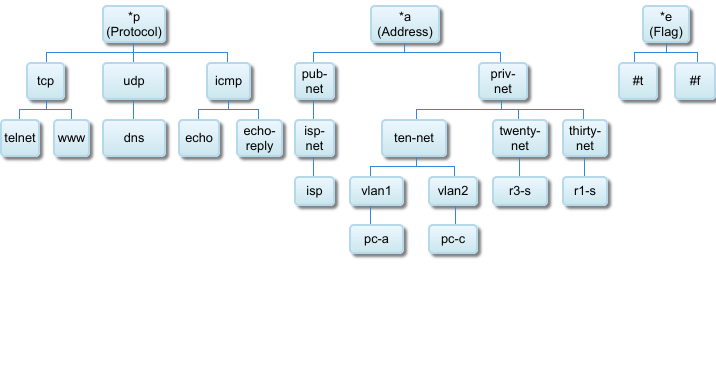
\includegraphics[width=\textwidth]
    {figures/hier.png}}
    \caption{\label{hier} Hierarchy of ranges}
\end{figure}

Values are leaves at the bottom of the trees. Note that even though all values are ranges, but some ranges are not necessarily values. Additionally, this data can be nicely translated to S-expression\footnote{This expressions is a \textit{forest}, which in turns is a list of \textit{trees}. We will describe trees and forests later on the in the implementation.}:
\begin{lstlisting}
((*p (tcp (telnet) (www))
     (udp (dns))
     (icmp (echo) (echo-reply)))
     
 (*a (pub-net  (isp-net (isp)))
     (priv-net (ten-net (vlan1 (pc-a))
                        (vlan2 (pc-c)))
               (twenty-net (r3-s))
               (thirty-net (r1-s))))
               
 (*e (#t) (#f)))
\end{lstlisting}

\subsection{Implementation of the firewall analyzer}
With the model in mind, we can translate each concept into its representation as S-expressions. A packet is a list of its values of the four fields (e.g. \code{(telnet isp isp #t)}). ACLs are lists of their entries. An entry is like a packet, but with ranges instead of values for its fields and an action attached to the beginning. For example, \code{(deny *p *a *a *e)} is the familiar "deny all" entry inserted implicitly at the end of each ACL. That much can help us define the first two high-level functions \code{entry-matcht} and \code{acl-mapo}. \code{entry-matcht} is a pseudo-function of \code{entry} and \code{pkt} and returns the result of the question "Does \code{pkt} match \code{entry}?". \code{acl-mapo} uses \code{entry-matcht} to process the packet \code{pkt} with the entries in \code{acl} and unifies \code{entry} with the one that the packet matches. Due to the implicit "deny all" at the end, every packet will match with an entry as long as it is well-formed.
\begin{lstlisting}
(define entry-matcht
  (lambda (entry pkt)
    (lambda (?)
      (fresh (eaction epkt)
        (== `(,eaction . ,epkt) entry)
        ((super*t epkt pkt) ?)))))

(define acl-mapo
  (lambda (acl pkt entry)
    (conde
     [(== '() acl)
      (== entry '[deny *p *a *a *e])
      (;; Ensures that the packet is well-formed
       (entry-matcht entry pkt)
       #t)]
     [(fresh (a d)
        (== `(,a . ,d) acl)
        (condo
         [(entry-matcht a pkt) (== a entry)]
         [else (acl-mapo d pkt entry)]))])))
\end{lstlisting}

To ask if a packet matches an entry is a question of determining whether the ranges in the entry cover the values in the packet. Therefore, the hierarchy in figure \ref{hier} is involved and for that we need \textbf{tree} processing. Trees are formally defined as the mutually recursive data structure where:
\begin{itemize}
    \item A tree is a pair of an arbitrary value (its \textbf{root node}) and a forest (its \textbf{children}) and
    \item A forest is a list of trees.
\end{itemize}

\begin{figure}
    {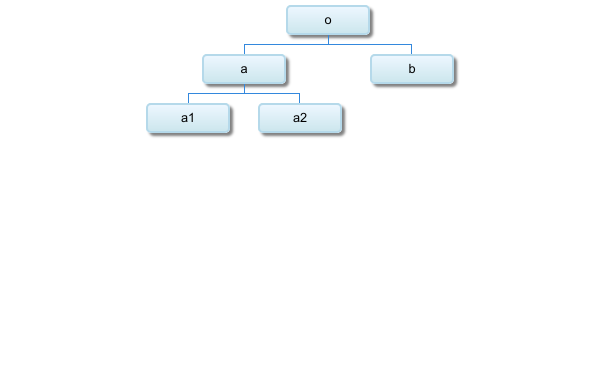
\includegraphics[width=\textwidth]
    {figures/example-tree.png}}
    \caption{\label{example-tree} Example tree}
\end{figure}

For instance, the tree in figure \ref{example-tree} is written in S-expression as \code{(o (a (a1) (a2)) (b))}. We define the tree find and forest find relations below. These two are also pseudo-functions because they need to communicate internally whether \code{sub} is found under a \code{tree} or \code{forest}.
\begin{lstlisting}
(define tree-forest-findt
  (lambda (sub)
    (letrec
        ([tree-findt
          (lambda (tree)
            (lambda (found?)
              (fresh (v u f g)
                (== tree `(,v . ,f))
                (== sub  `(,u . ,g))
                (condo
                 [(==t u v)
                  (== f g)
                  (== #t found?)]
                 [else
                  ((forest-findt f) found?)]))))]

         [forest-findt
          (lambda (forest)
            (lambda (found?)
              (conde
               [(== '() forest) (== #f found?)]
               [(fresh (a d)
                  (== `(,a . ,d) forest)
                  (condo
                   [(tree-findt a) (== #t found?)]
                   [else ((forest-findt d) found?)]))])))])

      (values tree-findt forest-findt))))

(define tree-findt
  (lambda (tree sub)
    (let-values ([(t _f) (tree-forest-findt sub)])
      (t tree))))

(define forest-findt
  (lambda (forest sub)
    (let-values ([(_t f) (tree-forest-findt sub)])
      (f forest))))
\end{lstlisting}

Finally, we define the relations to represent when a range subsumes a value. \code{supert} is the core, dealing with a single field. It finds the subtree with root \code{v1} in the hierarchy (which is always successful) and then find the leaf node \code{v2} under that subtree, the result of which is the result of the entire function. \code{super*t}, used by \code{entry-matcht} above, handles all four fields\footnote{However, \code{super*t} is defined on arbitrary lists so it can handle infinitely many fields should we want it to.}.
\begin{lstlisting}
(define supert
  (lambda (v1 v2)
    (lambda (?)
      (fresh (t1 _f1)
        (== t1 `(,v1 . ,_f1))
        ((forest-findt hier t1)     #t)
        ((tree-findt   t1   `(,v2)) ?)))))

(define super*t
  (lambda (e1 e2)
    (lambda (?)
      (conde
       [(== '() e1) (== '() e2) (== #t ?)]
       [(fresh (a1 d1 a2 d2)
          (== `(,a1 . ,d1) e1)
          (== `(,a2 . ,d2) e2)
          ((conjt (supert a1 a2)
                  (super*t d1 d2))
           ?))]))))
\end{lstlisting}

\subsection{Sample usage}
Our examples use the ACL below:
\begin{lstlisting}
(define acl100
  '([permit www  ten-net *a         *e]
    [permit tcp  pc-a    r3-s       *e]
    [deny   echo ten-net twenty-net *e]
    [permit icmp ten-net twenty-net *e]))
\end{lstlisting}

Given a packet \code{[echo pc-a r3-s #f]}, we can ask the question "Does acl100 block this packet?" with this query:
\begin{lstlisting}
(let ([pkt '[echo pc-a r3-s #f]])
      (run* (entry)
        (acl-mapo acl100 pkt entry)))
\end{lstlisting}
$\Rightarrow$ \code{((deny echo ten-net twenty-net *e))}

The matched entry is a deny, so indeed it was blocked. This is, however, not an exciting example because we can do the same thing with Packet Tracer. The interesting examples come from running the programs "backward". For example, we can ask which packets are blocked by acl100 (and by which entries):
\begin{lstlisting}
(run 10 (pkt entry)
      (fresh (?) (== `(deny . ,?) entry))
      (acl-mapo acl100 pkt entry))
\end{lstlisting}
$\Rightarrow$
\begin{lstlisting}
(((www isp isp #t)    (deny *p *a *a *e))
 ((www isp isp #f)    (deny *p *a *a *e))
 ((echo pc-a r3-s #t) (deny echo ten-net twenty-net *e))
 ((echo pc-a r3-s #f) (deny echo ten-net twenty-net *e))
 ((echo pc-c r3-s #t) (deny echo ten-net twenty-net *e))
 ((echo pc-c r3-s #f) (deny echo ten-net twenty-net *e))
 ((www isp pc-a #t)   (deny *p *a *a *e))
 ((www isp pc-a #f)   (deny *p *a *a *e))
 ((www isp pc-c #t)   (deny *p *a *a *e))
 ((www isp pc-c #f)   (deny *p *a *a *e)))
\end{lstlisting}

How to read this: packet \code{(www isp isp #t)} is blocked by the "deny all" entry, packet \code{(echo pc-a r3-s #t)} is blocked by the \code{(deny echo ten-net twenty-net *e)} entry, etc. Although the program works as expected, we found a glaring issue that even non-TCP packets can contain the established flag. I think fixing this should be easy, but chose not to do so for the simplicity of the code.

By restricting the entry parameter even more, we question the usefulness of each entry. For example, we can ask which function the final entry serves (if it even does anything).
\begin{lstlisting}
(run 1 (pkt entry)
  (fresh (?) (== '[permit icmp ten-net twenty-net *e] entry))
  (acl-mapo acl100 pkt entry))
\end{lstlisting}
$\Rightarrow$
\begin{lstlisting}
(((echo-reply pc-a r3-s #t)
  (permit icmp ten-net twenty-net *e)))
\end{lstlisting}

For the grand finale, we can ask the computer to synthesize an entry, given a specified behavior:
\begin{lstlisting}
(run 1 (missing)
      (fresh (acl e1 e2)
        (== `([permit www  ten-net *a         *e]
             [permit tcp  pc-a    r3-s       *e]
             ,missing
             [permit icmp ten-net twenty-net *e])
           acl)
        (fresh (?) (== `(deny . ,?)   e1))
        (fresh (?) (== `(permit . ,?) e2))
        (acl-mapo acl '[echo       pc-a r3-s #f] e1)
        (acl-mapo acl '[echo-reply pc-a r3-s #f] e2)))
\end{lstlisting}
And... miniKanren never returns an answer, at least with today's hardware. \fi
    \section{Conclusion}
\ifthesis
This paper presented the following contributions:
\begin{enumerate}
\item A technique of using "reified if" to express failure in a relational manner.
\item The implementation a miniKanren variant to help extract certain "modes" of a program.
\item A way of reformatting staticKanren's answers to make it look more like the source program.
\end{enumerate}
The result of these contributions is the language staticKanren containing (besides mode extraction) a better presentation of answers and a more elegant core enabled by the omission of infinite streams. Additionally, staticKanren programs look a lot more like Scheme program. Perhaps this fact might be beneficial in making miniKanren programs more appealing to Scheme users.

The goal of this thesis is to explore techniques of avoiding code duplication of positive and negative relations. We learned the important lesson that while failure can be easily expressed with reified goal constructors such as \code{condo}, the behavior of the program is almost impossible to preserve. The best solution to this problem suggested by this paper is to specify the two-way algorithm, run it through staticKanren, and manually modify the generated result if needed.

This solution is not ideal, particularly due to the additional framework in staticKanren. However, I believe that it is a necessary price to pay for the mechanization of negation while retaining utmost user flexibility. An alternative approach no explored here is to use constructive negation (\cite{chan}), although it seems significantly more complex to implement.

There is an interesting use case of staticKanren in Scheme program analysis. With the help of \code{condo} it is very easy to convert any Scheme program into staticKanren and extract its various modes. This application was not explored in the paper due to time constraint, but it would be a nice topic for future work.
\else
\fi
\else
    \ifthesis \section{Relational conditionals with pseudo-functions}\label{reif}
\subsection{The problem with conde}
Suppose we need to write a relation called \code{lookupo} to retrieve a variable's value in an environment. The task at first is just a straightforward transformation from the Scheme function \code{lookup}.
\begin{lstlisting}
(define lookup
  (lambda (x env)
    (let ([a (car env)])
      (cond
       [(eq? x (lhs a)) (rhs a)]
       [else (lookup x (cdr env))]))))

(define lookupo
  (lambda (x env t)
    (fresh (y b rest)
      (== `((,y ,b) . ,rest) env)
      (conde
       [(== y x) (== b t)]
       [(=/= y x) (lookupo x rest t)]))))
\end{lstlisting}

Later on we might need to actually handle the case where the variable is unbound instead of raising an error or fail. We update both definitions:
\begin{lstlisting}
(define lookup
  (lambda (x env)
    (cond
     [(null? env) #f]
     [else
      (let ([a (car env)])
        (cond
         [(eq? x (lhs a)) a]
         [else (lookup x (cdr env))]))])))

(define lookupo
  (lambda (x env t bound?)
    (conde
     [(== '() env) (== #f bound?)]
     [(fresh (y b rest)
        (== `((,y ,b) . ,rest) env)
        (conde
         [(== y x) (== #t bound?) (== b t)]
         [(=/= y x) (lookupo x rest t bound?)]))])))
\end{lstlisting}

So far so good: \code{lookup} only needs to add an input indicating whether the variable is bound; meanwhile for \code{lookup} we have to devise a special signal, namely \code{#f}, for the unbound case\footnote{There is technically a way to return multiple values in Scheme, but doing so would be lengthy and unconventional.}. However, a problem arises when we actually use the output signal:
\begin{lstlisting}
(define case1
  (lambda (x env)
    (cond
     [(lookup x env) => rhs]
     [else #f])))

(define case1o
  (lambda (x env out)
    (conde
     [(lookupo x env out #t)]
     [(lookupo x env 'unbound #f) (== #f out)])))
\end{lstlisting}

Why can we not use \code{else} in the second clause? The reason is that despite the similarity in appearance, \code{conde} does not process its clauses from top to bottom like \code{cond} does, so there can be no default case. As a result, programmers must always be prepared to append extra denials in lower \code{conde} clauses. This issue gets serious when the control flow is more complex:

\begin{lstlisting}
(define case2
  (lambda (x y env)
    (cond
     [(lookup x env) => rhs]
     [(lookup y env) => rhs]
     [else #f])))

(define case2o
  (lambda (x y env out)
    (conde
     [(lookupo x env out #t)]
     [(lookupo x env '? #f) (lookupo y env out #t)]
     [(lookupo x env '? #f) (lookupo y env '? #f)
      (== #f out)])))
\end{lstlisting}

The example above is still generous, as it is usual for relations to include four or more \code{conde} clauses. The number of extra denials exhibits quadratic growth, introducing opportunities for errors without any significant contribution to the meaning of the program. Fortunately, there is a simple way to deal with them using a technique inspired by \textcite{reif}. This solution relies on \textbf{pseudo-functions}.

\subsection{Pseudo-function and condo}
Pseudo-functions receive their results as arguments instead of returning them. To make sense of this concept, observe the following transformation (the "t" at the end denotes pseudo-functions, simply because it is too late to change):
\begin{lstlisting}
;; From function
(define bar (lambda (in) 'v))
;; To relation
(define baro (lambda (in out) (== out 'v)))
;; To pseudo-function...
(define bart (lambda (in) (lambda (out) (baro in out))))
;; ...which is equivalent to
(define bart (lambda (in) (lambda (out) (== out 'v))))
\end{lstlisting}

From a low-level point of view, a pseudo-function is a function which takes a single argument and return a goal. It can be seen that the act of returning values in functional programming is analogous to the act of unification in logic/relational programming. Moreover, a relation can be made to return whichever of its formal parameters, depending on the circumstances:
\begin{lstlisting}
;; From relation
(define conso (lambda (a d ls) (== `(,a . ,d) ls)))
;; To pseudo-function 1
(define cart (lambda (ls) (lambda (a) (fresh (d) (conso a d ls)))))
;; To pseudo-function 2
(define cdrt (lambda (ls) (lambda (d) (fresh (a) (conso a d ls)))))
;; To pseudo-function 3
(define const (lambda (a d) (lambda (ls) (conso a d ls))))
\end{lstlisting}
I have never encountered a situation where this is actually useful, since there is generally only one parameters deemed as the "output". It is worth noting that even though pseudo-functions act like pure functions, they can affect more than just the output. For instance, the goal \code{((cart x) a)} will always instantiate \code{x} to a pair if it is currently unknown.

Going back to the problem of conditionals, we first define two trivial pseudo-functions \code{truet} and \code{falset}, "returning" \code{#t} and \code{#f} respectively.

\begin{lstlisting}
(define truet (lambda () (lambda (?) (== #t ?))))
(define falset (lambda () (lambda (?) (== #f ?))))
\end{lstlisting}

Next, we define a single "primitive" pseudo-function similar to Scheme's \code{eq?}\footnote{Depending on the implementation, more primitive pseudo-functions may be defined using additional primitive constraints.}. This function relies on both \code{==} and \code{=/=} to correctly express two branches of the output.
\begin{lstlisting}
(define ==t
  (lambda (x y)
    (lambda (?)
      (conde
       [(== #t ?) (== x y)]
       [(== #f ?) (=/= x y)]))))
\end{lstlisting}

Next, we provide ways of creating more complex pseudo-functions from simpler ones, starting with \code{negt} (negation):
\begin{lstlisting}
(define negt
  (lambda (g)
    (lambda (?)
      (conde
       [(== #t ?) (g #f)]
       [(== #f ?) (g #t)]))))
\end{lstlisting}

From this, \code{=/=t} can be trivially derived:
\begin{lstlisting}
(define =/=t
  (lambda (x y) (negt (==t x y))))
\end{lstlisting}

Similarly, \code{conjt} (conjunction) and \code{disjt} (disjunction) are defined using macro:
\begin{lstlisting}
(define-syntax conjt
  (syntax-rules ()
    [(_) (truet)]
    [(_ g) g]
    [(_ g1 g2 gs ...)
     (lambda (?)
       (conde
        [(g1 #t) ((conjt g2 gs ...) ?)]
        [(== #f ?) (g1 #f)]))]))

(define-syntax disjt
  (syntax-rules ()
    [(_) (falset)]
    [(_ g) g]
    [(_ g1 g2 gs ...)
     (lambda (?)
       (conde
        [(== #t ?) (g1 #t)]
        [(g1 #f)  ((disjt g2 gs ...) ?)]))]))
\end{lstlisting}

This next example demonstrates conjunction:
\begin{lstlisting}
(run* (t x y z)
   ((conjt (==t x y)
           (==t y z))
    t))
\end{lstlisting}
$\Rightarrow$
\begin{lstlisting}
(((#f _.0 _.1 _.2) (=/= ((_.0 _.1))))
 (#t _.0 _.0 _.0)
 ((#f _.0 _.0 _.1) (=/= ((_.0 _.1)))))
\end{lstlisting}

Similarly, this example demonstrates disjunction:
\begin{lstlisting}
(run* (t x y z)
   ((disjt (==t x y)
           (==t y z))
    t))
\end{lstlisting}
$\Rightarrow$
\begin{lstlisting}
((#t _.0 _.0 _.1)
 ((#t _.0 _.1 _.1) (=/= ((_.0 _.1))))
 ((#f _.0 _.1 _.2) (=/= ((_.0 _.1)) ((_.1 _.2)))))
\end{lstlisting}

Finally, we can define the goal constructor \code{condo} -- the closest relational counterpart of \code{cond}. Keep in mind that \code{succeed} stands for the "do nothing" goal and \code{fail} stands for the "always fail" goal.
\begin{lstlisting}
(define-syntax condo
  (syntax-rules (else)
    [(_ [else]) succeed]
    [(_ [else g]) g]
    [(_ [else g1 g2 g* ...])
     (fresh () g1 g2 g* ...)]
    [(_ [test g* ...] c* ...)
     (conde
      [(test #t) g* ...]
      [(test #f) (condo c* ...)])]
    [(_) fail]))
\end{lstlisting}
\code{condo} is an interesting combinator because it uses two types of objects, pseudo-functions in the test positions and normal miniKanren goals in the bodies of each clause. The \code{else} keyword can be used to signify the default case; although it can be omitted, in which case the program fails when no clause matches. The example below demonstrates the use of \code{condo}:
\begin{lstlisting}
(run* (x y z)
  (condo
   [(==t x y) succeed]
   [(==t y z) succeed]
   [else (== x z)]))
\end{lstlisting}
$\Rightarrow$
\begin{lstlisting}
((_.0 _.0 _.1)
 ((_.0 _.1 _.1) (=/= ((_.0 _.1))))
 ((_.0 _.1 _.0) (=/= ((_.0 _.1)))))
\end{lstlisting}

We are now able to replace \code{lookupo} with the pseudo-function \code{lookupt}.
\begin{lstlisting}
(define lookupt
  (lambda (x env t)
    (lambda (bound?)
      (conde
       [(== '() env)
        (== #f bound?) (== t 'unbound)]
       [(fresh (y b rest)
          (== `((,y ,b) . ,rest) env)
          (condo
           [(==t y x) (== #t bound?) (== b t)]
           [else
            ((lookupt x rest t) bound?)]))]))))
\end{lstlisting}
Now the comparison between \code{case2} and \code{case2o} does not look so bad anymore.
\begin{lstlisting}
(define case2
  (lambda (x y env)
    (cond
     [(lookup x env) => rhs]
     [(lookup y env) => rhs]
     [else #f])))

(define case2o
  (lambda (x y env)
    (lambda (out)
      (condo
       [(lookupt x env out) succeed]
       [(lookupt y env out) succeed]
       [else (== #f out)]))))
\end{lstlisting}

Some readers may already be convinced to convert all of their relations to pseudo-functions. However, there are still some issues to address. Although hiding the control flow is great for readability, the downside is that there is no simple way to see what is done behind the layer of abstraction. As a result, it becomes easier to accidentally change the behavior of programs. Take for example this goal using \code{condo}:
\begin{lstlisting}
(fresh (x y)
  (condo
   [(==t 'a x) (== 'A y)]
   [(==t 'b x) (== 'B y)]
   [(==t 'c x) (== 'C y)]))
\end{lstlisting}
It is not clear that there is an issue with this code, because it looks so much like normal Scheme. The issue only shows itself when we expand the \code{condo}:
\begin{lstlisting}
(fresh (x y)
  (conde
   [(== 'a x) (== 'A y)]
   [(=/= 'a x) (== 'b x) (== 'B y)]
   [(=/= 'a x) (=/= 'b x) (== 'c x) (== 'C y)]))
\end{lstlisting}
Clearly, the additional denials in these \code{conde} clause are redundant since they are already mutually exclusive. Moreover, switching from \code{conde} to \code{condo} always means changing the way miniKanren's search work.

Reality has shown that serious miniKanren users who are conscious about their programs' behavior cannot afford \code{condo}, so we are once again stuck with lengthy, buggy \code{conde} clauses whose meaning cannot not be easily grasped. The next section addresses this issue by offering a way to verify the correctness of existing programs with \textbf{staticKanren}. \else \section{A firewall analysis assistant in miniKanren}\label{firewall}
\subsection{Our simplified model}
There are many types of firewalls, but for this work we will only consider networking firewalls defined by Access Control Lists (ACL). An ACL is a sequence of entries, each in turns defines a range of values to be compared against network packets. When an ACL processes a packet, it compares the packet against its entries from top to bottom until a matched entry is found, and an action specified by that entry is taken. For our purpose, we assume that actions can only be either \textit{permit} or \textit{deny}, the meaning of which will depend on the practical context.

Modeling is the most important aspect of this work. Although there is practical value in models that are close to how real life ACL works, they are not very simple to understand and to work with. Therefore, in this paper we will construct our own model simple enough to demonstrate the fundamental ideas.

In our model, a packet is simply a quadruple of values belonging to four fields: its protocol, its source address, its destination address and its flag. Correspondingly there are three high-level ranges (types of values):
\begin{itemize}
    \item \textbf{All protocols} (Denoted \code{*p}): A protocol is a specific format of data such as \code{tcp}, \code{udp}, \code{icmp}, etc.
    \item \textbf{All addresses} (Denoted \code{*a}): Although IPv4 addresses are predominantly used these days, we will assign symbolic values for addresses for simplicity. Examples can be \code{pc-a}, \code{isp}, etc.
    \item \textbf{All flags} (Denoted \code{*e}): A flag is a TCP field to determine the connection phase. There are only two Boolean values \code{#t} (established) and \code{#f} (not established).
\end{itemize}

There is actually a hierarchy of ranges to help in configuring ACL. The example hierarchy in figure \ref{hier} is global in this paper, but it can be customized depending on the specific use case (especially the addresses).

\begin{figure}
    {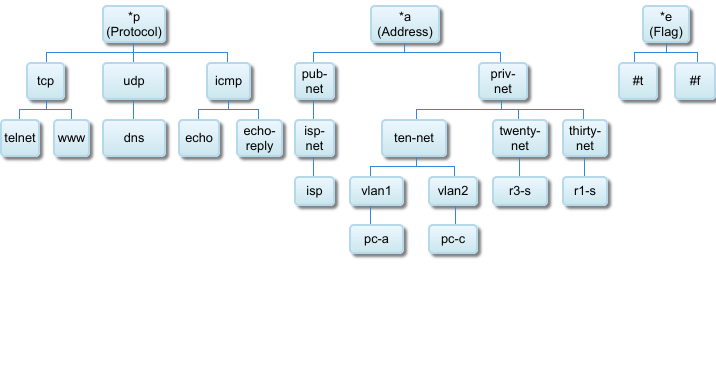
\includegraphics[width=\textwidth]
    {figures/hier.png}}
    \caption{\label{hier} Hierarchy of ranges}
\end{figure}

Values are leaves at the bottom of the trees. Note that even though all values are ranges, but some ranges are not necessarily values. Additionally, this data can be nicely translated to S-expression\footnote{This expressions is a \textit{forest}, which in turns is a list of \textit{trees}. We will describe trees and forests later on the in the implementation.}:
\begin{lstlisting}
((*p (tcp (telnet) (www))
     (udp (dns))
     (icmp (echo) (echo-reply)))
     
 (*a (pub-net  (isp-net (isp)))
     (priv-net (ten-net (vlan1 (pc-a))
                        (vlan2 (pc-c)))
               (twenty-net (r3-s))
               (thirty-net (r1-s))))
               
 (*e (#t) (#f)))
\end{lstlisting}

\subsection{Implementation of the firewall analyzer}
With the model in mind, we can translate each concept into its representation as S-expressions. A packet is a list of its values of the four fields (e.g. \code{(telnet isp isp #t)}). ACLs are lists of their entries. An entry is like a packet, but with ranges instead of values for its fields and an action attached to the beginning. For example, \code{(deny *p *a *a *e)} is the familiar "deny all" entry inserted implicitly at the end of each ACL. That much can help us define the first two high-level functions \code{entry-matcht} and \code{acl-mapo}. \code{entry-matcht} is a pseudo-function of \code{entry} and \code{pkt} and returns the result of the question "Does \code{pkt} match \code{entry}?". \code{acl-mapo} uses \code{entry-matcht} to process the packet \code{pkt} with the entries in \code{acl} and unifies \code{entry} with the one that the packet matches. Due to the implicit "deny all" at the end, every packet will match with an entry as long as it is well-formed.
\begin{lstlisting}
(define entry-matcht
  (lambda (entry pkt)
    (lambda (?)
      (fresh (eaction epkt)
        (== `(,eaction . ,epkt) entry)
        ((super*t epkt pkt) ?)))))

(define acl-mapo
  (lambda (acl pkt entry)
    (conde
     [(== '() acl)
      (== entry '[deny *p *a *a *e])
      (;; Ensures that the packet is well-formed
       (entry-matcht entry pkt)
       #t)]
     [(fresh (a d)
        (== `(,a . ,d) acl)
        (condo
         [(entry-matcht a pkt) (== a entry)]
         [else (acl-mapo d pkt entry)]))])))
\end{lstlisting}

To ask if a packet matches an entry is a question of determining whether the ranges in the entry cover the values in the packet. Therefore, the hierarchy in figure \ref{hier} is involved and for that we need \textbf{tree} processing. Trees are formally defined as the mutually recursive data structure where:
\begin{itemize}
    \item A tree is a pair of an arbitrary value (its \textbf{root node}) and a forest (its \textbf{children}) and
    \item A forest is a list of trees.
\end{itemize}

\begin{figure}
    {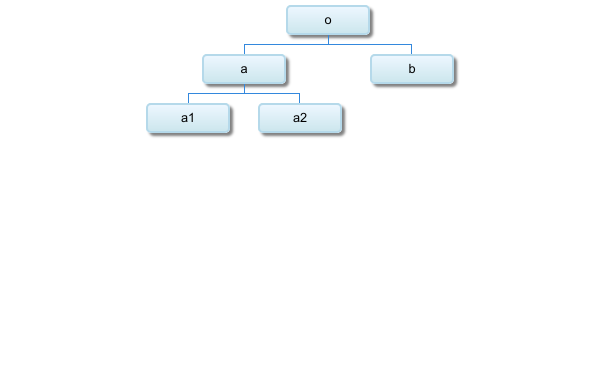
\includegraphics[width=\textwidth]
    {figures/example-tree.png}}
    \caption{\label{example-tree} Example tree}
\end{figure}

For instance, the tree in figure \ref{example-tree} is written in S-expression as \code{(o (a (a1) (a2)) (b))}. We define the tree find and forest find relations below. These two are also pseudo-functions because they need to communicate internally whether \code{sub} is found under a \code{tree} or \code{forest}.
\begin{lstlisting}
(define tree-forest-findt
  (lambda (sub)
    (letrec
        ([tree-findt
          (lambda (tree)
            (lambda (found?)
              (fresh (v u f g)
                (== tree `(,v . ,f))
                (== sub  `(,u . ,g))
                (condo
                 [(==t u v)
                  (== f g)
                  (== #t found?)]
                 [else
                  ((forest-findt f) found?)]))))]

         [forest-findt
          (lambda (forest)
            (lambda (found?)
              (conde
               [(== '() forest) (== #f found?)]
               [(fresh (a d)
                  (== `(,a . ,d) forest)
                  (condo
                   [(tree-findt a) (== #t found?)]
                   [else ((forest-findt d) found?)]))])))])

      (values tree-findt forest-findt))))

(define tree-findt
  (lambda (tree sub)
    (let-values ([(t _f) (tree-forest-findt sub)])
      (t tree))))

(define forest-findt
  (lambda (forest sub)
    (let-values ([(_t f) (tree-forest-findt sub)])
      (f forest))))
\end{lstlisting}

Finally, we define the relations to represent when a range subsumes a value. \code{supert} is the core, dealing with a single field. It finds the subtree with root \code{v1} in the hierarchy (which is always successful) and then find the leaf node \code{v2} under that subtree, the result of which is the result of the entire function. \code{super*t}, used by \code{entry-matcht} above, handles all four fields\footnote{However, \code{super*t} is defined on arbitrary lists so it can handle infinitely many fields should we want it to.}.
\begin{lstlisting}
(define supert
  (lambda (v1 v2)
    (lambda (?)
      (fresh (t1 _f1)
        (== t1 `(,v1 . ,_f1))
        ((forest-findt hier t1)     #t)
        ((tree-findt   t1   `(,v2)) ?)))))

(define super*t
  (lambda (e1 e2)
    (lambda (?)
      (conde
       [(== '() e1) (== '() e2) (== #t ?)]
       [(fresh (a1 d1 a2 d2)
          (== `(,a1 . ,d1) e1)
          (== `(,a2 . ,d2) e2)
          ((conjt (supert a1 a2)
                  (super*t d1 d2))
           ?))]))))
\end{lstlisting}

\subsection{Sample usage}
Our examples use the ACL below:
\begin{lstlisting}
(define acl100
  '([permit www  ten-net *a         *e]
    [permit tcp  pc-a    r3-s       *e]
    [deny   echo ten-net twenty-net *e]
    [permit icmp ten-net twenty-net *e]))
\end{lstlisting}

Given a packet \code{[echo pc-a r3-s #f]}, we can ask the question "Does acl100 block this packet?" with this query:
\begin{lstlisting}
(let ([pkt '[echo pc-a r3-s #f]])
      (run* (entry)
        (acl-mapo acl100 pkt entry)))
\end{lstlisting}
$\Rightarrow$ \code{((deny echo ten-net twenty-net *e))}

The matched entry is a deny, so indeed it was blocked. This is, however, not an exciting example because we can do the same thing with Packet Tracer. The interesting examples come from running the programs "backward". For example, we can ask which packets are blocked by acl100 (and by which entries):
\begin{lstlisting}
(run 10 (pkt entry)
      (fresh (?) (== `(deny . ,?) entry))
      (acl-mapo acl100 pkt entry))
\end{lstlisting}
$\Rightarrow$
\begin{lstlisting}
(((www isp isp #t)    (deny *p *a *a *e))
 ((www isp isp #f)    (deny *p *a *a *e))
 ((echo pc-a r3-s #t) (deny echo ten-net twenty-net *e))
 ((echo pc-a r3-s #f) (deny echo ten-net twenty-net *e))
 ((echo pc-c r3-s #t) (deny echo ten-net twenty-net *e))
 ((echo pc-c r3-s #f) (deny echo ten-net twenty-net *e))
 ((www isp pc-a #t)   (deny *p *a *a *e))
 ((www isp pc-a #f)   (deny *p *a *a *e))
 ((www isp pc-c #t)   (deny *p *a *a *e))
 ((www isp pc-c #f)   (deny *p *a *a *e)))
\end{lstlisting}

How to read this: packet \code{(www isp isp #t)} is blocked by the "deny all" entry, packet \code{(echo pc-a r3-s #t)} is blocked by the \code{(deny echo ten-net twenty-net *e)} entry, etc. Although the program works as expected, we found a glaring issue that even non-TCP packets can contain the established flag. I think fixing this should be easy, but chose not to do so for the simplicity of the code.

By restricting the entry parameter even more, we question the usefulness of each entry. For example, we can ask which function the final entry serves (if it even does anything).
\begin{lstlisting}
(run 1 (pkt entry)
  (fresh (?) (== '[permit icmp ten-net twenty-net *e] entry))
  (acl-mapo acl100 pkt entry))
\end{lstlisting}
$\Rightarrow$
\begin{lstlisting}
(((echo-reply pc-a r3-s #t)
  (permit icmp ten-net twenty-net *e)))
\end{lstlisting}

For the grand finale, we can ask the computer to synthesize an entry, given a specified behavior:
\begin{lstlisting}
(run 1 (missing)
      (fresh (acl e1 e2)
        (== `([permit www  ten-net *a         *e]
             [permit tcp  pc-a    r3-s       *e]
             ,missing
             [permit icmp ten-net twenty-net *e])
           acl)
        (fresh (?) (== `(deny . ,?)   e1))
        (fresh (?) (== `(permit . ,?) e2))
        (acl-mapo acl '[echo       pc-a r3-s #f] e1)
        (acl-mapo acl '[echo-reply pc-a r3-s #f] e2)))
\end{lstlisting}
And... miniKanren never returns an answer, at least with today's hardware. \fi
\fi


%\section{Applications}

%\section{Conclusion}

%References, this was marked with "r"
%---------------------------------------------------------------------------------------------------------------

%These two should always go together
\newpage

\begingroup 
% NO more line spacing for references
\linespread{1}

% Set spacing between bibliography spacing
\setlength\bibitemsep{\baselineskip}

% NO more hanging indentation for bibliograpy
\setlength{\bibhang}{0pt}

\section*{REFERENCES}
\phantomsection
\addcontentsline{toc}{section}{REFERENCES}

\printbibliography[heading=none]
\endgroup















\end{document}
